\section{Neural Networks}
\label{ch:neural_networks}

As mentioned the name neural network has prevailed despite being neither neural nor networks.
Initially having the brain as inspiration they are used to create more complex mappings than previous models.
In the following it is discussed what the motivation is behind this concept is and how networks are being trained to solve a variety of problems.

\subsection{Deep learning}
\label{ch:deep_learning}

Even though the universal approximation theorem shows that all continuous functions can be described using only one layer, in practice it is much more feasible to add multiple layers to our model to keep the necessary resources low.
Rolnick and Tegmark\cite{Rolnick2017} show that for single layered models the number of neurons grow exponentially with the number of variables of the input, whereas deep neural networks grow only linearly.

% TODO add some clues for notation
\begin{figure} \label{fig:nn}
    \centering
    \caption{ A neural network with three nodes as input, two hidden layers with five nodes each and an output layer with three nodes. The bias is added to each layer by prepending a one. Every node is, like the previous example calculated by the sum of the product of the previous layer and their respective weight. }
    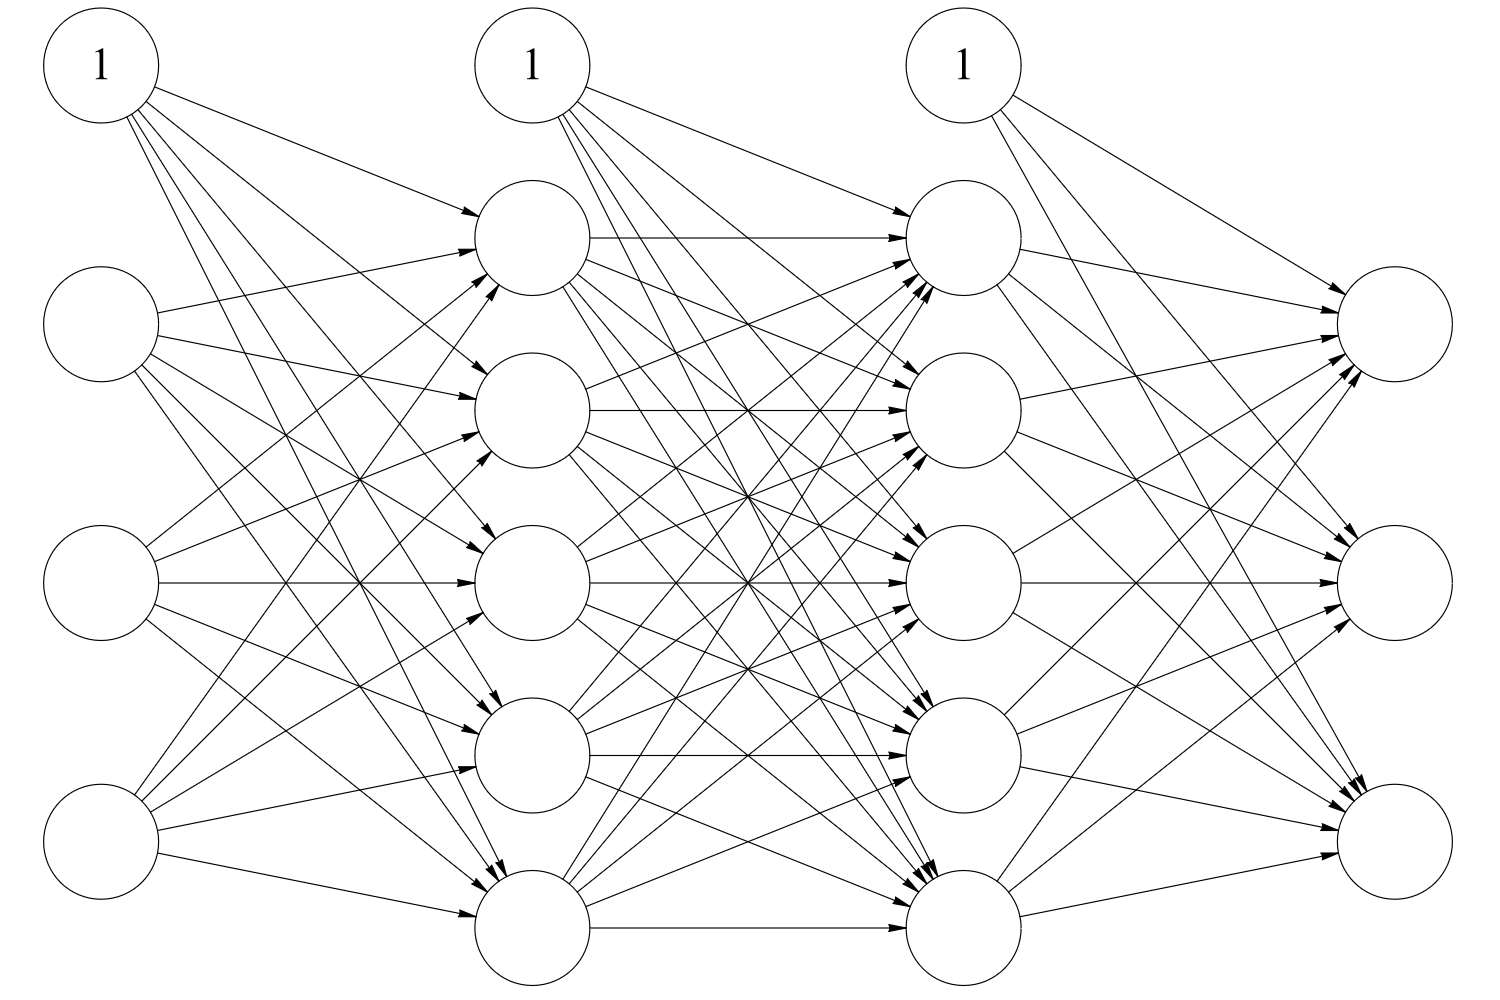
\includegraphics[width=0.6\textwidth]{images/2_nn_with_bias.png}
\end{figure}

Every node in figure~\ref{fig:nn} can be addressed using the notation $z^l_i$. $l$ being the number of the layer in which the node resides and $i$ being the index of the node.
Every weight $\theta^l_{i, j}$ can be addressed too; $l$ being the layer the weight points to, $i$ being the index of the node which is multiplied with the weight to influence the value of the node in layer $l$ with index $j$.
Thus we can describe every node as a result of:

\begin{equation} \label{eq:node_value}
    z^l_j = \sum^n_{i=0}z^{l-1}_i\theta^l_{i, j}
\end{equation}

$n$ being the number of nodes in the respective layer. Equation~\eqref{eq:node_value} can be vectorized with:

\begin{equation} \label{eq:node_value_vectorized}
    z^l = \theta^l z^{l-1}
\end{equation}

\subsection{Activation functions}

A problem with activations like the ones mentioned above are that they can come out as numbers of any size. Numerically this is very hard to control, so the nodes themselves are wrapped inside another function; this function is fittingly called the activation function.

\begin{figure} \label{fig:activation}
    \centering
    \begin{subfigure}[b]{0.3\textwidth}
        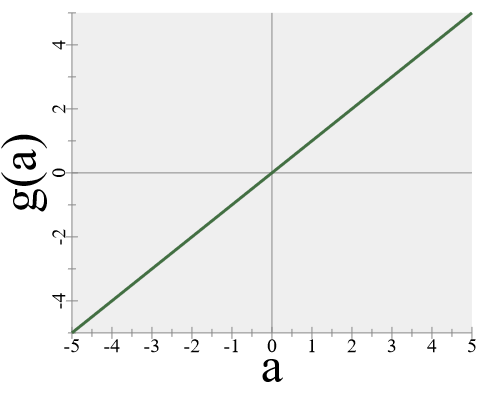
\includegraphics[width=\textwidth]{images/4_linear.png}
        \caption{Linear}
        \label{fig:activation_linear}
    \end{subfigure}
    \begin{subfigure}[b]{0.3\textwidth}
        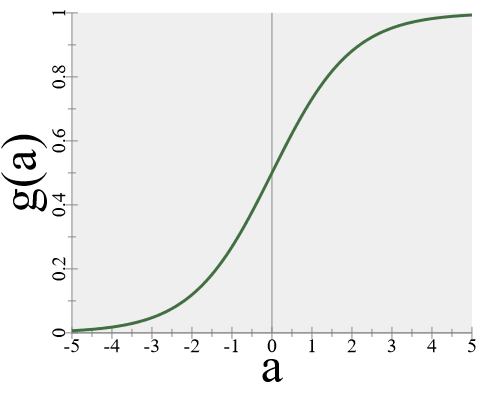
\includegraphics[width=\textwidth]{images/4_sigmoid.png}
        \caption{Logistic sigmoid}
        \label{fig:activation_sigmoid}
    \end{subfigure}
    \begin{subfigure}[b]{0.3\textwidth}
        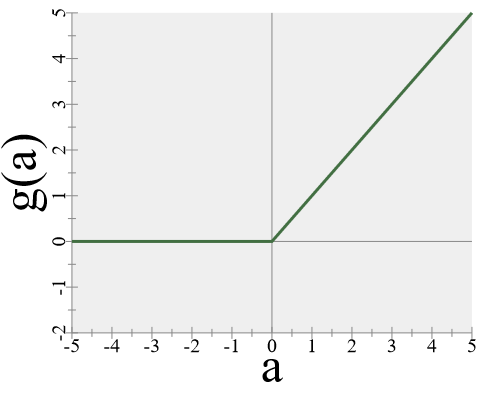
\includegraphics[width=\textwidth]{images/4_relu.png}
        \caption{ReLU}
        \label{fig:activation_relu}
    \end{subfigure}
    \caption{} % TODO maybe add some text to activation functions?
\end{figure}

Activation functions are used in different ways and give more possibilities to adjust yet new parameters to increase model performance.
Previously we intrinsically assumed the linear function shown in figure~\ref{fig:activation_linear} with the mapping $g(a) = a$.
The logistic sigmoid is often used in practice, because it creates a mapping of arbitrary numerical input and maps it into the interval $[0,1]$.
The rectified linear unit is much easier computationally and is recommended for use with most feedforward neural networks\cite[p.169]{Goodfellow2017}\cite{Glorot2011}.
Mathematical representations are shown in equation~\eqref{eq:sigmoid_relu}

\begin{equation}
    \label{eq:sigmoid_relu}
    \begin{split}
        Sigmoid: f(x) & = \frac{1}{1 + \exp^{-x}} \\ ReLU: f(x) & = max(0, x)
    \end{split}
\end{equation}

The usage of those functions can vary as well; e.g. it is common for the logistic sigmoid to have a threshold to not fire at all if a certain value (say 0.5) is not reached.

By the introduction of activation functions equations~\eqref{eq:node_value} and \eqref{eq:node_value_vectorized} extend to:

\begin{equation} \label{eq:activation}
    a^l_j = \sigma(z^l_j) = \sigma(\sum^n_{i=0}z^{l-1}_i\theta^l_{i, j})
\end{equation}

With the respective vectorized equation being:

\begin{equation} \label{eq:activation_vectorized}
    a^l = \sigma(z^l) = \sigma(\theta^l z^{l-1})
\end{equation}

There are a variety of different activation functions, with these two being the most prominent, but there are other for different purposes too. The selection of the activation function and possibly a corresponding threshold are another hyper parameter which has to be chosen prior to training.

\subsection{Backpropagation}

Using gradient descent~\eqref{eq:gradient_descent} we can not update all parameters in all layers, since it only considers updating the parameters of the last layer.
Since the last layer is a function of the respective previous layer, we can propagate the calculated error of the last layer to it and update the weights and bias respectively. This conjuncture is true for any layer, except the input layer (which does not need to be updated after all).
Equations used to perform this are\footnote{The following equations are derived using \cite[p.733]{StuartRussell2018}, \cite[p.197]{Goodfellow2017} and \cite{Nielsen2015, ch.2}}:

\begin{equation}\label{eq:output_error}
    \varDelta^L = \nabla_a L \odot \sigma'(z^L)
\end{equation}
\begin{equation}\label{eq:hidden_error}
    \varDelta^l = ((\theta^{l+1})^T \varDelta^{l+1}) \odot \sigma'(z^l)
\end{equation}
\begin{equation} \label{eq:backprop_update}
    \theta_{i+1} := \theta_i - \eta \varDelta
\end{equation}

Equation~\eqref{eq:output_error} describes the error calculated in the output layer. We define our network with $L$ layers, thus the output layer is always described by index $L$.
$\odot$ is the Hadamard operator. It is used to multiply tensors elementwise, which is useful in this case, because it prevents us from having to transform one of the vectors into a diagonal matrix, making the calculation a bit less complicated.
Equation~\eqref{eq:output_error} is a direct result of applying the chain rule of multivariate calculus to the derivation of the loss function performed in the last layer.
We already mentioned that gradient descent is performed by taking the derivative on the loss function in equation~\eqref{eq:sgd_mse_here}.
Because between the input used in the loss function and the output of the preceding layer an activation function is implemented, the chain rule has to be applied to the gradient of the loss.

\begin{equation}\label{eq:proof_loss_chain_rule}
    \frac{\partial L}{\partial z^L_j} = \frac{\partial L}{\partial a^L_j}\frac{\partial a^L_j}{\partial z^L_j}
\end{equation}

By pointing out that $\frac{\partial L}{\partial a^L_i}$ is just a non vectorized form of $\nabla_a L$ and $\frac{\partial a^L_i}{\partial z^L_i}$ of $\sigma'(z^L)$ the equivalence becomes apparent.

Equation~\eqref{eq:hidden_error} can be rewritten to:
\begin{equation}
    \varDelta^l_i = \frac{\partial L}{\partial z^l_i} = \sum_{j=0}^n (\frac{\partial L}{\partial z^{l+1}_j}\frac{\partial z^{l+1}_j}{\partial z^l_i})
\end{equation}

$n$ being the number of nodes in the subsequent layer. Since $\frac{\partial L}{\partial z^{l+1}_i} = \varDelta^{l+1}_i$ it follows:

\begin{equation} \label{eq:hidden_error_intermediate}
    \frac{\partial L}{\partial z^l_i} = \sum_{j=0}^n (\varDelta^{l+1}_j \frac{\partial z^{l+1}_j}{\partial z^{l}_i})
\end{equation}

We also know that:
\begin{equation}
    \begin{split}
    z^{l+1}_j & = \sum_{i=0}^n \theta^{l+1}_{i,j} a^l_i = \sum_{i=0}^n \theta^{l+1}_{i, j} \sigma(z^l_i) \\
    \frac{\partial z_j^{l+1}}{\partial z_i^l} & = \theta^{l+1}_{i,j} \sigma'(z^l_j)
    \end{split}
\end{equation}

So we can substitute the terms in equation~\eqref{eq:hidden_error_intermediate} to:
\begin{equation}
    \frac{\partial L}{\partial z^l_i} = \sum_{j=0}^n (\varDelta^{l+1}_j \theta^{l+1}_{i,j} \sigma'(z_j^l))
\end{equation}

Which is again just a non vectorized form of equation~\eqref{eq:hidden_error}.

Equation~\eqref{eq:hidden_error} is subsequently performed on each layer until $l=0$ is reached and a $\varDelta$ is calculated for each parameter in $\theta$ which are applied using equation~\eqref{eq:backprop_update}.
This manner of propagating backwards gave this algorithm the prominent name of back propagation (short for "backward propagation of error"\cite{Rumelhart1986}).

\subsection{Generalization}

The task of every machine learning algorithm is to generalize.
After feeding the model with data it has seen, it should also perform well on data it has never seen before.
This distinguishes machine learning from optimization problems (which could be solved by e.g. the Newton-Raphson method).

Generalization is not granted, because of problems called overfitting and underfitting.
For example a model trained for a classification task might overfit by correctly predicting classes for training examples, but may to fail to do so on new data.
This indicates that the model memorized the training examples.
There are some things which can be done to solve this issue.
Giving the model more data to train on is one solution, which is shown by Banko and Brill\cite{Banko2001} and famously commented on by Halevy, Norvig and Pereira in their article "The Unreasonable Effectiveness of Data"\cite{Halevy2009}.
Adding a multitude of data is not always possible, since data generation may be costly, so some compromises may have to be made to solve this issue.

Another option is to reduce features of the training data; seemingly unintuitive at first, it becomes apparent that abundant features do not add much information to an image. For example to recognize a handwritten digit, a lot of more parameters have to be adjusted if a high resolution image with hundreds of thousands of pixels are fed into the model, where under a thousand would suffice\cite{Nielsen2015}.

On the other hand the problem of underfitting is as problematic as is overfitting.
When the model does not even get sufficient results on the training data, the problem is called underfitting.
If this is the case the model may have to be adjusted to adjust more parameters or the data may not be fitting to the problem after all.
For equations~\eqref{eq:universal_approx} and \eqref{eq:hypothesis} to be true for a reasonable model a mapping of the input to the expected output has at least to be somewhat comprehensible.

Before using these techniques to train a model to recognize mechanical symbols, the respective data has to be generated first.
